%! TEX program = pdflatex
%% Mauricio Caceres Bravo <mauricio.caceres.bravo@gmail.com>

%----------------------------------------------------------------------
\documentclass{article}

\usepackage[summary]{brownpreamble}
\usepackage{etoc}
\setcounter{tocdepth}{3}

\renewcommand{\subsectionmark}[1]{\markboth{#1}{}}
\renewcommand\sectiontype{Lecture \thesection:\ }
\lhead{\color{light-gray} \itshape Math Camp Aug 23, 2021 -- Lecture \thesection}
\rhead{\color{light-gray} \itshape \thesubsection. \leftmark}
\setcounter{section}{4}
% \renewcommand\SetHideLevel{1pt}

%----------------------------------------------------------------------
\begin{document}
\displayoptions

% ---------------------------------------------------------------------
\section{Constrained Optimization, Integration}
\label{sec:constrained_optimization_integration}

\localtableofcontents

% ---------------------------------------------------------------------
\subsection{Constrained Optimization}
\label{sub:constrained_optimization}

The general problem of constrained optimization can be written as
\begin{equation}\label{eq:lecture5_main_problem}
  \max_{x \in \mathbb{R}^N} f(x)
  \quad
  g(x) \le b
  \quad
  h(x) = c
\end{equation}


$f: \mathbb{R}^N \to \mathbb{R}$ is a real-valued function, $g: \mathbb{R}^N \to \mathbb{R}^K$, $h: \mathbb{R}^N \to \mathbb{R}^M$ are vector-vaued functions, and $b \in \mathbb{R}^K$ and $c \in \mathbb{R}^M$ are constants. Recall
\begin{align*}
  g(x) \le b \equiv g_k(x) \le b_k
  \quad\text{and}\quad
  h(x) = c \equiv h_m(x) \le c_m
\end{align*}

The function $f$ is called the \keyword{objective}, the functions that comprise $g$ are called the \keyword{inequality constraints}, and the functions that comprise $h$ are called \keyword{equality constraints}.

\begin{example}
  What is the maximum of $f(x) = x^2$ on $[0, 1]$? We can write this as
  \begin{align*}
    \max_{x \in \mathbb{R}} f(x)
    \quad
    g(x) \le b
  \end{align*}

  where $g: \mathbb{R} \to \mathbb{R}^2$ is given by $g(x) = (-x, x)$ and $b = (0, 1)$. A more common way to write this, however, is
  \begin{align*}
    \max_{x \in \mathbb{R}} x^2
    \quad\text{s.t.}\quad
    0 \le x \le 1
  \end{align*}

  In this case, the maximum occurs at $x = 1$ (note $f(x)$ is strictly increasing).
\end{example}

\subsubsection{One Equality Constraint}
\label{ssub:one_equality_constraint}

Suppose that we only have a single equality constraint:
\begin{align*}
  \max_{x \in \mathbb{R}^N} f(x)
  \quad
  h(x) = c
\end{align*}

with $c \in \mathbb{R}$ some scalar. With unconstrained optimization, we look for candidate extrama by solving for $x$ using the FOC. In this case, however, solving for the FOC doesn't immediately help because the candidate points might not be in the constraint. What to do?
\begin{itemize}[label=$\bullet$]
  \item Suppose that we could solve for $x_i$ for some $i$ explicitly as a function of $c$ and the other variables. WLOG let this be $x_1$; that is, given $h(x) = c$ we find $\varphi$ s.t.
    \begin{align*}
      x_1 = \varphi(x_{-1})
      \iff
      h(x) = c
    \end{align*}

    Then we can pug in $x_1$ and we have
    \begin{align*}
      \max_{x \in \mathbb{R}^N} f(\varphi(x_{-1}), x_{-1})
    \end{align*}

    The FOC for this transformed problem is
    \begin{equation}
      \label{eq:lecture5_foc_lagrangian_exampe}
      0
      =
      D f(\varphi(x_{-1}^*), x_{-1}^*)
      =
      D_{x_1} f(\varphi(x_{-1}^*), x_{-1}^*) D_{x_{-1}} \varphi(x_{-1}^*)
      +
      D_{x_{-1}} f(\varphi(x_{-1}^*), x_{-1}^*)
    \end{equation}

    and any $x_{-1}^*$ satisfying \Cref{eq:lecture5_foc_lagrangian_exampe} for the unconstrained problem gives a candidate point of the constrained problem: $(\varphi(x_{-1}^*), x_{-1}^*)$ with $\varphi(x_{-1}^*) = x_1^*$.

  \item Given the above, if there was a general way of finding $\varphi$ we'd be good. This is not possible, but we don't really need to solve for $\varphi$ \textit{explicitly}. Looking at the FOC, all the expressions are computable except for $D_{x_{-1}} \varphi(x_{-1}^*)$. Looking back at the constraint, if we plug in $\varphi$, we can write any $x^*$ satisfies
    \begin{align*}
      h(\varphi(x_{-1}^*), x_{-1}^*) - c = 0
    \end{align*}

    and now you should be reminded of the IFT!

  \item In other words, even when we cannot find an explicit expression for $\varphi$, we know implicitly such a function exists. Following the theorem, we can compute
    \begin{align*}
      D_{x_{-1}} \varphi(x_{-1}^*) = - (D_{x_1} h(x^*))^{-1} (D_{x_{-1}} h(x^*))
    \end{align*}

    Plugging this into \Cref{eq:lecture5_foc_lagrangian_exampe}, we find
    \begin{align*}
      0
      &
      =
      - D_{x_1} f(x^*) (D_{x_1} h(x^*))^{-1} (D_{x_{-1}} h(x^*))
      +
      D_{x_{-1}} f(x^*)
      \\
      D_{x_{-1}} f(x^*)
      &
      =
      \left[
        D_{x_1} f(x^*) (D_{x_1} h(x^*))^{-1}
      \right]
      D_{x_{-1}} h(x^*)
    \end{align*}

    Let $\lambda_1 \equiv D_{x_1} f(x^*) (D_{x_1} h(x^*))^{-1}$ and we have any optimum must satisfy
    \begin{align*}
      D_{x_{-1}} f(x^*)
      &
      =
      \lambda_1 D_{x_{-1}} h(x^*)
    \end{align*}

    This should be a very familiar expression!

  \item Indeed, what we just found is almost exactly the method of Lagrangians you know and love. What's missing? Well, remember $1$ was chosen arbitrarily, so we can write down the above expression $2, \ldots, N$ and find the corresponding expression with $\lambda_2, \ldots, \lambda_N$. However, the gradients at $x^*$ will not  change, which implies that $\lambda_i = \lambda_j$. Hence we can simply write
    \begin{align*}
      D_x f(x^*)
      =
      \lambda D_x h(x^*)
    \end{align*}

    for any local optimum, which is exactly the method of Lagrange multipliers.
\end{itemize}

% xx TODO: Graphical intuition. Function expanding in unit circle? Maybe UMP in BC?

\begin{example}
  Consider $f(x, y) = \sqrt{x \cdot y}$, $h(x, y) = x^2 + y^2$, and $c = 1$. Solve
  \begin{align*}
    \max_{x, y} (xy)^{1/2}
    \quad\text{s.t.}\quad x^2 + y^2 = 1
  \end{align*}

  We know that $(Df) = \lambda (Dh)$ for some  $\lambda$, or
  \begin{align*}
    \begin{bmatrix}
      \dfrac{1}{2} x^{-1/2} y^{1/2}
      \\
      \dfrac{1}{2} x^{1/2} y^{-1/2}
    \end{bmatrix}
    &
    =
    \lambda
    \begin{bmatrix}
      2x
      \\
      2y
    \end{bmatrix}
    \\
    \begin{bmatrix}
      x^{-1/2} y^{1/2}
      \\
      x^{1/2} y^{-1/2}
    \end{bmatrix}
    &
    =
    4
    \lambda
    \begin{bmatrix}
      x
      \\
      y
    \end{bmatrix}
    \\
    \dfrac{x^{-1/2} y^{1/2}}{x^{1/2} y^{-1/2}}
    &
    =
    \dfrac{x}{y}
    \\
    x^2
    &
    =
    y^2
  \end{align*}

  The last step is to use the constraint, which must hold at the optimum as well:
  \begin{align*}
    x^2 + x^2 = 1
    \implies
    x = y = \sqrt{1/2}
    \quad\text{or}\quad
    x = y = - \sqrt{1/2}
  \end{align*}

  Note that we can't mix and match roots here lest the objective be $\sqrt{}$ a negative number.
\end{example}

\subsubsection{Multiple Equality Constraints}
\label{ssub:multiple_equality_constraints}

\begin{theorem}[Lagrange Multipliers]\label{thm:lecture5_lagrangian}
  Let $f: \mathbb{R}^N \to \mathbb{R}$ and  $h: \mathbb{R}^N \to \mathbb{R}^M$ be  continuously differentiable and $x^*$ be a solution to
  \begin{equation}
    \max_{x \in \mathbb{R}^N} f(x)
    \quad\text{s.t.}\quad
    h(x) = c
    \label{eq:lecture5_max_lagrangian_theorem}
  \end{equation}

  for a given $c \in \mathbb{R}^M$. If $\rank(Dh(x^*)) = M \le N$ (this rank condition is called a \keyword{non-degenerate constraint qualification};  why is a NDCQ required?\footnote{There cannot be more non-redundant constraints than there are variables, lest the problem have no solution!}) then $\exists \lambda^* \in \mathbb{R}^M$ s.t.
  \begin{align*}
    Df(x^*)
    & =
    Dh(x^*) \lambda^*
    \\
    \dfrac{\partial f(x^*)}{\partial x_k}
    & =
    \sum^{M}_{i = 1}
    \dfrac{\partial h_i(x^*)}{\partial x_k} \lambda_i^*
  \end{align*}

  $\lambda^* = (\lambda_1^*, \ldots, \lambda_M^*)$ are called \keyword{Lagrange multipliers}.
\end{theorem}

Note the above is equivalent to stating that if $x^*$ solves \Cref{eq:lecture5_max_lagrangian_theorem} then $\exists \lambda^*$ s.t. $(x^*, \lambda^*)$ satisfy the FOC for
\begin{equation}
  \mathcal{L}(x, \lambda)
  =
  f(x) - (h(x) - c) \lambda
\end{equation}

In the above equation $\mathcal{L}$ is called the \keyword{Lagrangian}, so the result from \Cref{thm:lecture5_lagrangian} that $Df(x^*) = Dh(x^*) \lambda^*$ is referred to as the FOC for the Lagrangian.
\begin{example}
  Let $f(x, y, z) = xyz$, $h_1(x, y, z) = x^2 + y^2$, $h_2(x, y, z) = x + z = 1$, and $c_1 = c_2 = 1$. Solve
  \begin{align*}
    \max_{x, y, z} f(x, y, z)
    &
    \quad\text{s.t.}\quad
    h(x, y, z) = c
    \\
    \max_{x, y, z} xyz
    &
    \quad\text{s.t.}\quad
    \begin{bmatrix}
      x^2 + y^2
      \\
      x + z
    \end{bmatrix}
    =
    \begin{bmatrix}
      1 \\ 1
    \end{bmatrix}
  \end{align*}

  Now we can apply the theorem:
  \begin{align*}
    \begin{bmatrix}
      yz \\ xz \\ xy
    \end{bmatrix}
    &
    =
    \begin{bmatrix}
      2x & 1
      \\
      2y & 0
      \\
      0  & 1
    \end{bmatrix}
    \begin{bmatrix}
      \lambda_1 \\ \lambda_2
    \end{bmatrix}
    \\
    xy
    &
    =
    \lambda_2
    \\
    \dfrac{xz}{2y}
    &
    =
    \lambda_1
    \\
    yz
    &
    =
    \dfrac{x^2z}{y} + xy
    \\
    y^2z
    &
    =
    x^2z + xy^2
  \end{align*}

  To finish we need to leverage the constraints: $z = x - 1$ and $y^2 = 1 - x^2$, so
  \begin{align*}
    (1 - x^2) (1 - x)
    &
    =
    x^2 (1 - x) + x (1 - x^2)
    \\
    0
    &
    =
    (1 - x - 3x^2) (1 - x)
  \end{align*}

  The solutions are given by $x = \left(1, \dfrac{1 \pm \sqrt{13}}{6}\right)$. Note that $x = 1$ cannot be a solution. In this case, $y = z = 0$ (this yields an objective of $0$, which we can readily check this is not a $\max$, but it is also an issue for how we solved the problem, where $y \ne 0$l is required). For the other two points:
  \begin{align*}
    x = \dfrac{1 + \sqrt{13}}{6}
    \quad
    z = \dfrac{5 - \sqrt{13}}{6}
    \quad
    y
    = - \sqrt{1 - \dfrac{14 + 2 \sqrt{13}}{36}}
    = - \dfrac{\sqrt{22 - 2 \sqrt{13}}}{6}
    \\
    x = \dfrac{1 - \sqrt{13}}{6}
    \quad
    z = \dfrac{5 + \sqrt{13}}{6}
    \quad
    y
    = - \sqrt{1 - \dfrac{14 - 2 \sqrt{13}}{36}}
    = - \dfrac{\sqrt{22 + 2 \sqrt{13}}}{6}
  \end{align*}

  (technically we get $4$, but the other two give a negative value for the objective, which is even smaller than $0$). With some tedious algebra (or plugging numbers into a computer) you find the function is maximized at the second point.
\end{example}
- 
\subsubsection{Inequality Constraints}
\label{ssub:inequality_constraints}

The trick is to realize we can think of inequality constraints as either
\begin{enumerate}
  \item \keyword{Binding}, that is, the optimum occurs along the boundary of the constraint. In this case we can treat them as equality constraints.

  \item \keyword{Non-binding}, in which case we can de facto ignore them.
\end{enumerate}

In other words, we can solve a problem with inequality constraints in almost the exact way we would a problem with equality constraints. Consider $\max_x f(x)$ s.t. $g(x) \le b$; one way to approach this:
\begin{itemize}[label=$\bullet$]
  \item Solve for $x^*: D f(x^*) = D g(x^*) \lambda$ like in a constrained problem assuming $g(x^*) = b$.
  \item Solve for $x^*: D f(x^*) = 0$ like in an unconstrained problem and check $g(x^*) < b$.
\end{itemize}

Once you have all the candidate points, check which is largest to determine the $\max$.
\begin{example}
  Consider maximizing $f(x, y) = \sqrt{xy}$ subject to $x + y \le 1$, $x, y \ge 0$.
  \begin{align*}
    Df(x, y)
    =
    \begin{bmatrix}
      \dfrac{1}{2} x^{-1/2} y^{1/2}
      \\
      \dfrac{1}{2} x^{1/2} y^{-1/2}
    \end{bmatrix}
    &
    =
    \begin{bmatrix}
      1
      \\
      1
    \end{bmatrix}
    \lambda
    =
    Dg(x, y) \lambda
    \\
    x & = y
  \end{align*}

  assuming  $x + y = 1$ at the optimum (note that if $x$ or $y$ are $0$ then $f(x, y) = 0$, which we can readily check is not a $\max$).  Here the candidate point is $(x, y) = (1/2, 1/2)$; now for the unconstrained problem, we note that $f$ is strictly increasing if $x, y > 0$, which means that any such point cannot be an unconstrained $\max$ (we can increase either $x$ or $y$ slightly and make the objective bigger). To recap:
  \begin{itemize}[label=$\bullet$]
    \item Solving assuming binding constraints we find $x = 0$ or $y = 0$ cannot be $\max$, and the Lagrange multiplier method  gives $(x, y) = (1/2, 1/2)$ as a possible maximum.

    \item Solving assuming non-binding constraints yields no solution.
  \end{itemize}

  Hence the only candidate point is $(x, y) = (1/2, 1/2)$.
\end{example}

% ---------------------------------------------------------------------
\subsection{Karush-Khun-Tucker (KKT) Conditions}
\label{sub:karush_khun_tucker_kkt_conditions}

\begin{theorem}[Karush-Khun-Tucker]\label{thm:lecture5_kkt}
  Let $f: \mathbb{R}^N \to \mathbb{R}$ be a real-valued function, $g: \mathbb{R}^N \to \mathbb{R}^K$, $h: \mathbb{R}^N \to \mathbb{R}^M$ vector-valued functions, and $b \in \mathbb{R}^K$ and $c \in \mathbb{R}^M$ constants. Suppose that $x^*$ is such that the constraint qualification is satisfied (non-degenerate) and that it solves
  \begin{align*}
    \max_{x \in \mathbb{R}^N} f(x^*)
    \quad
    \text{s.t.}
    \quad
    g(x^*) \le b
    \quad
    h(x^*) = c
  \end{align*}

  Then there exist $\mu \in \mathbb{R}^K_{+}, \lambda \in \mathbb{R}^M_{+}$ (non-negative Lagrange multipliers) s.t.
  \begin{enumerate}
    \item $Df(x^*) = Dg(x^*) \mu + Dh(x^*)\lambda$. This is still the first order condition of the Lagrangian; in this case,
      \[
        \mathcal{L}(x, \mu, \lambda) = f(x) - (g(x) - b)\mu - (h(x) - c) \lambda
      \]

    \item $(g_j(x^*) - b_j) \mu_j = 0$ for each $j = 1, \ldots, K$; this is called the \keyword{complementary slackness} condition.
  \end{enumerate}
\end{theorem}

Complementary slackness states that either the constraint binds with equality or that we can ignore it for the purposes of the FOC (i.e. either $g_j(x^*) = b$ or the corresponding $\mu_j = 0$). Note as we did when solving equality constraints, we typically have to leverage the fact that $h(x^*) = c$ and $g(x^*) \le b$ to arrive at a solution.

\begin{remark}
  The result of the above theorem is often known as the Kuhn-Tucker conditions, named after two mathematicians who showed the theorem in in the 1950s. However, Karush had already proven this result more than a decade earlier in his (apparently unpublished) masters' thesis.
\end{remark}

\subsubsection{Second Order Conditions}
\label{ssub:second_order_conditions}

Consider the problem in \Cref{eq:lecture5_main_problem} and suppose the functions are twice continuously differentiable, so the Lagrangian
\begin{align*}
  \mathcal{L}(x, \mu, \lambda) = f(x) - (g(x) - b)\mu - (h(x) - c) \lambda
\end{align*}

is twice continuously differentiable as well. Suppose $(x^*, \mu^*, \lambda^*)$ is s.t. $x^*$ is a solution to the problem and the KKT conditions are satisfied. Further suppose the constraints $g_1, \ldots, g_L$ are binding and the other $K - L$ constrains are non-binding. Then the Hessian of $\mathcal{L}$ with respect to $x$ is negative definite on the set
\begin{align*}
  V = \Fset{v: D \widetilde{g}(x^*) v = 0 \quad\text{and}\quad Dh(x^*) v = 0}
\end{align*}

with $\widetilde{g} = (g_1, \ldots, g_L)$. That is,
\begin{align*}
  v^T D^2_x (x^*, \mu^*, \lambda^*) v < 0
\end{align*}

for any $v \in V$. To check this condition, consider the \keyword{bordered Hessian}:
\begin{align*}
  H
  =
  \begin{bmatrix}
    0                    & 0        & D \widetilde{g}(x^*)^T \\
    0                    & 0        & D h(x^*)^T \\
    D \widetilde{g}(x^*) & D h(x^*) & D^2_x \mathcal{L}(x^*, \mu^*, \lambda^*)
  \end{bmatrix}
\end{align*}

You will note the bordered Hessian is basically the Hessian of the Lagrangian, but it is so-called because it looks like we are ``bordering'' $D^2_x \mathcal{L}$ with $D \widetilde{g}, Dh$. In any case, it is sufficient to check that the last $N - L - M$ leading principal minors of $H$:
\begin{itemize}[label=$\bullet$]
  \item For a $\max$, their determinants alternate signs, with the sign of the $(2(L + M) + 1)$th principal minor equal to $(-1)^{L + M + 1}$ (note the last $N - L - M$ leading principal minors are from $2(L + M) + 1$ to $2(L + M) + (N - L - M) = N + L + M$).
  \item For a $\min$, all the signs of their determinant equal $(-1)^{L + M}$.
\end{itemize}

You will note we are discarding the first $2(L + M)$ leading principal minors. Why?\footnote{The bordered Hessian cannot be  positive or negative definite due to the  matrix of  zeros in the top left corner (second derivatives with respect to the multipliers are a $0$). That discards checking the first $L + M$ leading principal minors. What about the next? Intuitively, we can think that binding conditions impose restrictions of parameters. Remember we motivated our sketch of the proof of the Lagrange multiplier method by invoking the IFT. Why did we do this? Because if for each constraint we express a variable in terms  of the others, we can solve the modified unconstrained problem. In other words, each constraint removes a variable from the problem, and there goes the other $L + M$ degrees of freedom.}

\subsubsection{Application to Economics}
\label{ssub:application_to_economics}

Consider a consumer with wealth $w > 0$ maximizing Cobb-Douglas utility $U(x, y) = x^\alpha y^{1 - \alpha}$ for goods $x, y \in \mathbb{R}$ with prices $p_x, p_y$ such that $x, y \ge 0$, $p_x, p_y > 0$.
\begin{align*}
  \max_{x, y} x^{\alpha} y^{1 - \alpha}
  \quad\text{s.t.}\quad
  x, y \ge 0
  \quad\text{and}\quad
  p_x x + p_y y \le w
\end{align*}

Note that $f(x, y) = x^\alpha y^{1 - \alpha}$, $g(x, y) = (-x, -y, p_x x + p_y y)$, and $b = (0, 0, w)$. We know from \Cref{thm:lecture5_kkt} that any maximum satisfies
\begin{align*}
  \begin{bmatrix}
    \alpha x^{\alpha - 1} y^{1- \alpha}
    \\
    (1 - \alpha) x^{\alpha} y^{- \alpha}
  \end{bmatrix}
  &
  =
  \begin{bmatrix}
    -1 & 0 & p_x \\
    0 & -1 & p_y
  \end{bmatrix}
  \begin{bmatrix}
    \mu_1 \\ \mu_2 \\ \mu_3
  \end{bmatrix}
\end{align*}

and $\mu_1 x = \mu_2 y = (p_x x + p_y y - w) \mu_3 = 0$. Let us consider cases: If
$x, y \ne 0$ then $\mu_1 = \mu_2 = 0$ and from the FOC we find
\begin{align*}
  \dfrac{\alpha x^{\alpha - 1} y^{1 - \alpha}}{(1 - \alpha) x^{\alpha} y^{- \alpha}}
  &
  =
  \dfrac{p_x}{p_y}
  \\
  \alpha p_y y
  &
  =
  (1 - \alpha) p_x x
\end{align*}

If $p_x x + p_y y < w$ then since $f$ is strictly increasing in either argument, we can find some $\varepsilon$ s.t. $p_x (x + \varepsilon) + p_y (y + \varepsilon) < w$ but $f(x + \varepsilon, y + \varepsilon) > f(x, y)$. Therefore the constraint is binding, and
\begin{align*}
  w
  &
  =
  \dfrac{\alpha}{1 - \alpha} p_y y + p_y y
  \\
  y
  &
  =
  \dfrac{(1 - \alpha) w}{p_y}
  \\
  x
  &
  =
  \dfrac{\alpha w}{p_y}
\end{align*}

Note if $x$ or $y$ are $0$ then the objective is $0$, which is lower than the objective when both $x, y > 0$ (as is the case above). Hence the only candidate point is given by
\begin{align*}
  (x, y)
  =
  \left(
  \dfrac{(1 - \alpha) w}{p_y}, \dfrac{\alpha w}{p_y}
  \right)
\end{align*}

In this case, the Lagrangian was
\begin{align*}
  \mathcal{L}(x, \mu)
  =
  x^\alpha y^{1 - \alpha}
  -
  x \mu_1
  -
  y \mu_2
  -
  (p_x x + p_y y - w) \mu_3
\end{align*}

Note here only the budget constraint is binding, so the bordered Hessian is
\begin{align*}
  \begin{bmatrix}
    0    & p_x & p_y \\
    p_x  & \alpha (\alpha - 1) x^{\alpha - 2} y^{1 - \alpha} & \alpha (1 - \alpha) x^{\alpha - 1} y^{- \alpha} \\
    p_y  & \alpha (1 - \alpha) x^{\alpha - 1} y^{- \alpha} & - \alpha (1 - \alpha) x^{\alpha} y^{-\alpha - 1}
  \end{bmatrix}
\end{align*}

Hence we have two variables and one binding constraint, so we check the last $2 - 1 = 1$ leading principal minors, which is the third leading principal minor, or just the matrix itself. The determinant is
\begin{align*}
  &
  0 \cdot \det
  \begin{bmatrix}
    \alpha (\alpha - 1) x^{\alpha - 2} y^{1 - \alpha} & \alpha (1 - \alpha) x^{\alpha - 1} y^{- \alpha} \\
    \alpha (1 - \alpha) x^{\alpha - 1} y^{- \alpha} & - \alpha (1 - \alpha) x^{\alpha} y^{-\alpha - 1}
  \end{bmatrix}
  \\
  &
  -
  p_x \cdot \det
  \begin{bmatrix}
    p_x  & \alpha (1 - \alpha) x^{\alpha - 1} y^{- \alpha} \\
    p_y  & - \alpha (1 - \alpha) x^{\alpha} y^{-\alpha - 1}
  \end{bmatrix}
  \\
  &
  +
  p_y \cdot \det
  \begin{bmatrix}
    p_x  & \alpha (\alpha - 1) x^{\alpha - 2} y^{1 - \alpha} \\
    p_y  & \alpha (1 - \alpha) x^{\alpha - 1} y^{- \alpha}
  \end{bmatrix}
  \\
  &
  =
  -
  p_x \cdot
  \left[
    - p_x \alpha (1 - \alpha) x^{\alpha} y^{-\alpha - 1}
    - p_y \alpha (1 - \alpha) x^{\alpha - 1} y^{- \alpha}
  \right]
  \\
  &
  +
  p_y \cdot
  \begin{bmatrix}
    p_x
    \alpha (1 - \alpha) x^{\alpha - 1} y^{- \alpha}
    +
    p_y
    \alpha (1 - \alpha) x^{\alpha - 2} y^{1 - \alpha}
  \end{bmatrix}
  \\
  &
  >
  0
\end{align*}

Finally, $L + M + 1 = 1 + 1 = 2$, so $(-1)^2 > 0$ means the determinant of the  3rd leading principal minor must be positive for a $\max$, and that is exactly what we found.

% ---------------------------------------------------------------------
\subsection{Envelope Theorem}
\label{sub:envelope_theorem}

Consider the function
\begin{align*}
  f(x; \theta) = x^\theta - x
\end{align*}

for $\theta \in (0, 1)$. From the FOC, $\theta x^{\theta - 1} = 1$, and we can parametrize the maximum for any value of $\theta$, $x^*(\theta) = \theta^{1/(1 - \theta)}$.
\begin{align*}
  f(x^*(\theta); \theta)
  =
  (x^*(\theta))^\theta - x^*(\theta)
  =
  \theta^{\theta /(1 - \theta)}
  -
  \theta^{1 /(1 - \theta)}
\end{align*}

If we are interested in how $f$ changes with respect to $\theta$, we can take this monster derivative. However, I'm too lazy to look up how to differentiate $\theta^\theta$, so instead I will do some wrangling. Note
\begin{align*}
  \dfrac{d}{d\theta}
  f(x^*(\theta); \theta)
  =
  \left(
    \partial_x f(x^*(\theta); \theta)
  \right) \dfrac{d x^*(\theta)}{d \theta}
  +
  \partial_{\theta} f(x^*(\theta); \theta)
\end{align*}

From the FOC, however, we know $\partial_x f(x^*(\theta); \theta) = 0$ for each $\theta$, meaning (writing just $x^*$ for ease of notation),
\begin{align*}
  \dfrac{d}{d\theta} f(x^*; \theta)
  =
  \partial_{\theta} f(x^*; \theta)
  =
  \partial_{\theta}
  \Big(
    \exp(\theta \log(x))
    +
    x
  \Big)_{x = x^*}
  =
  (x^*)^\theta \log(x^*)
\end{align*}

This trick of leveraging the FOC to obtain the derivative of the optimized objective with respect to a parameter is called the \keyword{envelope theorem}.  Graphically, we can see that
\begin{figure}[H]
  \centering
  \caption{Graphical Illustration of the Envelope Theorem}
  \label{fig:graphical_illustration_of_the_envelope_theorem}
  \begin{tikzpicture}
    \begin{axis}[name=plot1
      ,title={}
      ,width=9cm
      ,height=8cm
      ,ymin=0
      ,ymax=0.7
      ,xmin=0
      ,xmax=1
      ,domain=0:1
      ,ylabel=$f(x)$
      ,xlabel=$x$
    ]
      \addplot [smooth, samples = 200, opacity = 0.3] {x^(0.25) - x};
      \addplot [smooth, samples = 200, opacity = 0.3] {x^(0.333) - x};
      \addplot [smooth, samples = 200]                {x^(0.5) - x};
      \addplot [smooth, samples = 200, opacity = 0.3] {x^(0.667) - x};
      \addplot [smooth, samples = 200, opacity = 0.3] {x^(0.75) - x};
      \addplot [only marks, mark=*] coordinates {
        (0.1574901, 0.4724704)
        (0.19232,   0.3852174)
        (0.25,      0.25)
        (0.2963803, 0.147968)
        (0.3164062, 0.1054688)
      };
      \draw [->, >=latex] (axis cs:0.2, 0.55) -- (axis cs:0.16, 0.48);
      \node[above] at (axis cs:0.2, 0.55) {$f(x^*; \theta)$};
      \node[name=A1] at (axis cs:0.1574901, 0.4724704) {};
      \node[name=B1] at (axis cs:0.19232,   0.3852174) {};
      \node[name=C1] at (axis cs:0.25,      0.25)      {};
      \node[name=D1] at (axis cs:0.2963803, 0.147968)  {};
      \node[name=E1] at (axis cs:0.3164062, 0.1054688) {};
    \end{axis}

    \begin{axis}[name=plot2
      ,title={}
      ,at={($(plot1.east) + (0.5cm, 0)$)}
      ,anchor=west
      ,width=9cm
      ,height=8cm
      ,ymin=0
      ,ymax=0.7
      ,xmin=0
      ,xmax=1
      ,domain=0.15:0.9
      ,ylabel={$f(x^*(\theta), \theta)$}
      ,xlabel=$\theta$
    ]
    \addplot [smooth] {x^(x/(1 - x)) - x^(1/(1 - x))};
      \addplot [only marks, mark=*] coordinates {
        (0.25, 0.4724704)
        (0.333,0.3852174)
        (0.5,  0.25)
        (0.667,0.147968)
        (0.75, 0.1054688)
      };
      \node[name=A2] at (axis cs:0.25, 0.4724704) {};
      \node[name=B2] at (axis cs:0.333,0.3852174) {};
      \node[name=C2] at (axis cs:0.5,  0.25)      {};
      \node[name=D2] at (axis cs:0.667,0.147968)  {};
      \node[name=E2] at (axis cs:0.75, 0.1054688) {};
    \end{axis}
    \draw [dashed] (A1) -- (A2);
    \draw [dashed] (B1) -- (B2);
    \draw [dashed] (C1) -- (C2);
    \draw [dashed] (D1) -- (D2);
    \draw [dashed] (E1) -- (E2);
  \end{tikzpicture}
\end{figure}

In $x$--$\theta$ space, we can see that $f(x^*(\theta), \theta)$ \textit{\textbf{envelops}} $f(x, \theta)$ at each $(x^*(\theta), \theta)$ (hence the name).
\begin{figure}[H]
  \centering
  \caption{Graphical Illustration of the Envelope Theorem Ctd.}
  \label{fig:graphical_illustration_of_the_envelope_theorem_ctd}
  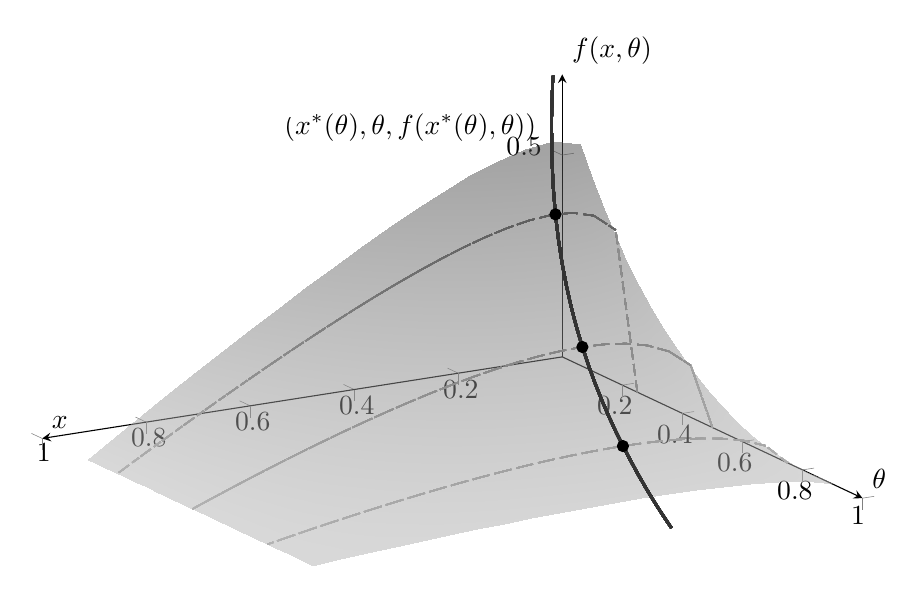
\begin{tikzpicture}
      \begin{axis}[name=plot1
        ,view={150}{30}
        ,width=12cm
        ,height=8cm
        ,zmin=0
        ,zmax=0.7
        ,xmin=0
        ,xmax=1
        ,ymin=0
        ,ymax=1
        ,ylabel=$\theta$
        ,xlabel=$x$
        ,zlabel={$f(x, \theta)$}
        ,xlabel style={anchor=south west}
        ,colormap={whiteblack}{color(0cm)  = (black!30); color(1cm) = (black)}
        ,axis lines=center
        ,xlabel style={anchor=south west}
        ,ylabel style={anchor=south west}
        ,zlabel style={anchor=south west}
        ,tick align=outside
        % ,clip=false
      ]
      \addplot3 [
        surf
        ,shader=interp
        ,fill opacity=0.5
        ,samples=20
        ,domain=0:1
        ,y domain=0.15:0.9
        % ,on layer=foreground
      ] {x^y-x};
      \addplot3[
        variable=t
        ,mesh
        ,domain=0:1
        ,color=black!80
        ,line width=1pt
      ] ({t^(1/(1 - t))},t,{t^(t/(1 - t)) - t^(1/(1 - t))});
      \addplot3[variable=t, mesh, dashed, opacity=0.8, domain=0:1, line width=0.5pt, on layer=foreground] (t,0.25,{t^0.25 - t});
      \addplot3[variable=t, mesh, dashed, opacity=0.8, domain=0:1, line width=0.5pt, on layer=foreground] (t,0.5,{t^0.5 - t});
      \addplot3[variable=t, mesh, dashed, opacity=0.8, domain=0:1, line width=0.5pt, on layer=foreground] (t,0.75,{t^0.75 - t});
      \addplot3 [only marks, mark=*] coordinates {
        (0.1574901, 0.25, 0.4724704)
        (0.25,      0.5,  0.25)
        (0.3164062, 0.75, 0.1054688)
      };
      \node at (axis cs:0.35, 0.1, 0.675) {$(x^*(\theta), \theta, f(x^*(\theta), \theta))$};
      \end{axis}
  \end{tikzpicture}
\end{figure}

\begin{theorem}[Envelope Theorem]
  Let $f: \mathbb{R}^N \times \Theta \to \mathbb{R}$ and $h: \mathbb{R}^M \to \mathbb{R}^N$ be continuously differentiable and $(x^*(\theta), \lambda^*(\theta))$ satisfy the FOC of the Lagrangian for the optimization problem at a given $\theta \in \Theta$:
  \begin{align*}
    \max_x f(x; \theta) \quad\text{s.t.}\quad h(x; \theta) = c
  \end{align*}

  The \keyword{value function} is the maximized value of the objective at each $\theta$, given by
  \begin{align*}
    V(\theta) \equiv f(x^*(\theta); \theta)
  \end{align*}

  If $V(\theta)$ is continuously differentiable at $\theta$ then
  \begin{align*}
    D_{\theta} V(\theta)
    &
    =
    \Big[
      D_{\theta} f(x; \theta)
      +
      \lambda
      D_{\theta} h(x; \theta)
    \Big]_{(x, \lambda) = (x^*(\theta), \lambda^*(\theta))}
    \\
    \dfrac{\partial V(\theta)}{\partial \theta_k}
    &
    =
    \dfrac{\partial f(x^*(\theta), \theta)}{\partial \theta_k}
    +
    \lambda^*(\theta) \dfrac{\partial g(x^*(\theta), \theta)}{\partial \theta_k}
  \end{align*}
\end{theorem}

Note that in our example, there is no constraint so the second term in the theorem is just $0$. (Alternatively, if $\theta$ does not appear in the constraint, the second term drops out of the expression as well.)

\subsubsection{Application to Economics}
\label{ssub:application_to_economics}

Consider a consumer minimizing expenditures subject to a minimum utility level $u$, with utility function $U(x, y) = x^\alpha y^{1 - \alpha}$ for goods $x, y \in \mathbb{R}$ with prices $p_x, p_y$ such that $x, y \ge 0$, $p_x, p_y > 0$.
\begin{align*}
  \min_{x, y} p_x x + p_y y
  \quad\text{s.t.}\quad
  x^{\alpha} y^{1 - \alpha} \ge u
\end{align*}

We can see that if the constraint is not binding at $(x, y)$, that is, $x^{\alpha} y^{1 - \alpha} > u$ then $\exists \varepsilon > 0$ s.t.  $(x- \varepsilon)^{\alpha} (y - \varepsilon)^{1 - \alpha} > u$. Since $p_x (x - \varepsilon) + p_y(y - \varepsilon) < p_x x + p_y y$, this point cannot be a minimum. Thus the constraint is binding, and we can apply the envelope theorem. The value function of this problem is called the \keyword{expenditure function}, given by
\begin{align*}
  e(p_x, p_y, u) = p_x x(p_x, p_y, u) + p_y y(p_x, p_y, u)
\end{align*}

with $x(\cdot), y(\cdot)$ the so-called Hicksian demand functions. We can see that to find gradient of the expenditure function with respect to price we can apply the envelope theorem! Noting $p_x, p_y$ are not in the constraint,
\begin{align*}
  D_{(p_x, p_y)} e(p_x, p_y, u)
  =
  \begin{bmatrix}
    x(p_x, p_y, u) \\ y(p_x, p_y, u)
  \end{bmatrix}
\end{align*}

% ---------------------------------------------------------------------
\subsection{Integration}
\label{sub:integration}

\subsubsection{Motivation and Definition}
\label{ssub:motivation_and_definition}

The motivation for integration is the problem of finding the area under a curve:
\begin{figure}[!ht]
  \centering
  \caption{Area Under $f(x)$}
  \label{fig:area_under_f_x_}
  \begin{tikzpicture}
    \begin{axis}[name=plot1
      %,title=
      ,width=12cm
      ,height=8cm
      ,ymin=0
      ,ymax=3
      ,xmin=0
      ,xmax=6
      ,domain=0:5.5
      ,ylabel=$f(x)$
      ,xlabel=$x$
      ,clip=false
    ]
    \addplot [smooth, name path = A, samples = 100] {x^(0.5)};
    \addplot [smooth, name path = B] {0};
    \addplot [color = shadecolor, opacity = 0.75] fill between[of = A and B];
    \node[below] at (axis cs:0, 0) {$a$};
    \node[below] at (axis cs:5.5, 0) {$b$};
    \end{axis}
  \end{tikzpicture}
\end{figure}

The strategy is to approximate the area under the curve with continuously tighter refinements:
\begin{figure}[H]
  \centering
  \caption{Approximate Area Under $f(x)$}
  \label{fig:approximate_area_under_f_x_}
  \begin{tikzpicture}
    \begin{axis}[name=plot1
      %,title=
      ,width=12cm
      ,height=8cm
      ,ymin=0
      ,ymax=3
      ,xmin=0
      ,xmax=6
      ,domain=0:5.5
      ,ylabel=$f(x)$
      ,xlabel=$x$
      ,clip=false
    ]
    \addplot [smooth, name path = A, samples = 100] {x^(0.5)};
    \addplot [smooth, name path = B] {0};
    \addplot [only marks, mark=*] coordinates {
      (0.5, 0.7071068)
      (1.5, 1.224745)
      (2.5, 1.581139)
      (3.5, 1.870829)
      (4.5, 2.12132)
      (5.5, 2.345)
    };
    \draw [-] (axis cs:0, 0) -- (axis cs:0, 0.707) -- (axis cs:0.5, 0.707) -- (axis cs:0.5, 0);
    \draw [-] (axis cs:0.5, 0) -- (axis cs:0.5, 1.225) -- (axis cs:1.5, 1.225) -- (axis cs:1.5, 0);
    \draw [-] (axis cs:1.5, 0) -- (axis cs:1.5, 1.581) -- (axis cs:2.5, 1.581) -- (axis cs:2.5, 0);
    \draw [-] (axis cs:2.5, 0) -- (axis cs:2.5, 1.871) -- (axis cs:3.5, 1.871) -- (axis cs:3.5, 0);
    \draw [-] (axis cs:3.5, 0) -- (axis cs:3.5, 2.121) -- (axis cs:4.5, 2.121) -- (axis cs:4.5, 0);
    \draw [-] (axis cs:4.5, 0) -- (axis cs:4.5, 2.345) -- (axis cs:5.5, 2.345) -- (axis cs:5.5, 0);

    \draw [-, opacity=0, name path = C]
      (axis cs:0, 0.707)   --
      (axis cs:0.5, 0.707) --
      (axis cs:0.5, 1.225) --
      (axis cs:1.5, 1.225) --
      (axis cs:1.5, 1.581) --
      (axis cs:2.5, 1.581) --
      (axis cs:2.5, 1.871) --
      (axis cs:3.5, 1.871) --
      (axis cs:3.5, 2.121) --
      (axis cs:4.5, 2.121) --
      (axis cs:4.5, 2.345) --
      (axis cs:5.5, 2.345);
    % pattern = north west lines
    \addplot [color = shadecolor, opacity = 0.75]
      fill between[of = C and B];

    \node[below] at (axis cs:0, 0) {$a$};
    \node[below] at (axis cs:5.5, 0) {$b$};
    \end{axis}
  \end{tikzpicture}
\end{figure}

The above approximation is given by
\begin{align*}
  \text{Area below $f$ from $a$ to $b$}
  \approx
  \sum^{m}_{i = 1} (x_i - x_{i - 1}) f(x_i)
\end{align*}

We can intuit that as our approximations become tighter, in the limit, we will recover the area under the curve exactly. Let us do this formally.
\begin{definition}
  Let $[a, b]$ be an interval on $\mathbb{R}$. A \keyword{partition} $P_m$ is a finite set of points $\set{x_0, \ldots, x_m}$ s.t.
  \begin{align*}
    a = x_0 \le x_1 \le \ldots \le x_{m - 1} \le x_m
  \end{align*}

  We denote $x_{i} - x_{i - 1} = \Delta x_i$.
\end{definition}

\begin{definition}
  Let $P_m$ be a partition of $[a, b]$; $P_n$ is a refinement of $P_m$ if $P_m \subseteq P_n$.
\end{definition}

\begin{definition}
  Let $f: [a, b] \to \mathbb{R}$ be bounded on $[a, b]$ and for any partition $P_m$ define
  \begin{align*}
    U_i & \equiv \sup_{x \in (x_{i - 1}, x_i)} f(x)
    \\
    L_i & \equiv \inf_{x \in (x_{i - 1}, x_i)} f(x)
    \\
    U(P_m, f) & \equiv \sum^{m}_{i = 1} U_i \Delta x_i
    \\
    L(P_m, f) & \equiv \sum^{m}_{i = 1} L_i \Delta x_i
  \end{align*}

  $U$ and $L$ are called the \keyword{upper Riemann sum} and \keyword{lower Riemann sum} of the partition $P_m$, respectively.
\end{definition}

\begin{definition}
  Let $f: [a, b] \to \mathbb{R}$ and consider $\mathcal{P}$ the set of all possible partitions of the interval $[a, b]$.
  \begin{align*}
    \inf_{P_m \in \mathcal{P}} U(P_m, f)
  \end{align*}

  is called the \keyword{upper Riemann integral} and
  \begin{align*}
    \sup_{P_m \in \mathcal{P}} L(P_m, f)
  \end{align*}

  is called the \keyword{lower Riemann integral}. If they are equal then $f$ is \keyword{Riemann integrable} on $[a, b]$  and the \keyword{Riemann integral} of $f$ is denoted
  \begin{align*}
    \int_{a}^{b} f(x) dx
    =
    \inf_{P_m \in \mathcal{P}} U(P_m, f)
    =
    \sup_{P_m \in \mathcal{P}} L(P_m, f)
  \end{align*}
\end{definition}

\begin{theorem}
  $f: [a, b] \to \mathbb{R}$ is Riemann integrable iff $\forall \varepsilon > 0 ~~ \exists P_m$ s.t. $U(P_m, f) - L(P_m, f) < \varepsilon$.
\end{theorem}

\begin{theorem}
  Let $f: [a, b] \to \mathbb{R}$ and $P_n$ be a refinement of $P_m$. Then
  \begin{align*}
    U(P_n, f) \le U(P_m, f)
    \quad\text{and}\quad
    L(P_n, f) \ge L(P_m, f)
  \end{align*}
\end{theorem}

\subsubsection{Properties and Theorems}
\label{ssub:properties_and_theorems}

Some useful properties of Riemann integrals (given $f, g: [a, b] \to \mathbb{R}$)
\begin{itemize}[label=$\bullet$]
  \item Order of integration:
    \[
      \int_{a}^{b} f(x) dx
      =
      - \int_{b}^{a} f(x) dx
    \]

  \item Zero-width interval:
    \[
      \int_{a}^{a} f(x) dx
      =
      0
    \]

  \item Constant multiple:
    \[
      \int_{a}^{b} c f(x) dx
      =
      c \int_{a}^{b} f(x) dx
    \]

  \item Sum and difference:
    \[
      \int_{a}^{b} (f \pm g)(x) dx
      =
      \int_{a}^{b} f(x) dx
      \pm
      \int_{a}^{b} g(x) dx
    \]

  \item Sum over intervals:
    \[
      \int_{a}^{b} f(x) dx
      +
      \int_{b}^{c} f(x) dx
      =
      \int_{a}^{c} f(x) dx
    \]

  \item Domination: If $f(x) \le g(x)$ for each $x \in [a, b]$ then
    \[
      \int_{a}^{b} f(x) dx
      \le
      \int_{a}^{b} g(x) dx
    \]

  \item Upper and lower bounds: If $L \le f(x) \le M$ for each $x \in [a, b]$ then
    \[
      L(a - b)
      \le
      \int_{a}^{b} f(x) dx
      \le
      U(a - b)
    \]
\end{itemize}

\begin{theorem}
  Let $f: [a, b] \to \mathbb{R}$ be Riemann integrable on $[a, b]$ and $g: f([a, b]) \to \mathbb{R}$ be a continuous function. Then $g \circ f$ is Riemann integrable on $[a, b]$.
\end{theorem}

\begin{corollary}
  Let $f, g: [a, b] \to \mathbb{R}$ be Riemann integrable on $[a, b]$. Then
  \begin{itemize}[label=$\bullet$]
    \item $f \cdot g$ is Riemann integrable on $[a, b]$.

    \item $|f|$ is Riemann integrable on $[a, b]$.
  \end{itemize}
\end{corollary}

\begin{theorem}[Jensen's Inequality]
  Let $f: [a, b] \to \mathbb{R}$ be Riemann integrable on $[a, b]$ and take $g: \mathbb{R} \to \mathbb{R}$.
  \begin{itemize}[label=$\bullet$]
    \item If $g$ is convex then $\displaystyle\int_{a}^{b} g(f(x)) dx \ge g\left(\int_{a}^{b} f(x) dx\right)$.

    \item If $g$ is concave then $\displaystyle\int_{a}^{b} g(f(x)) dx \le g\left(\int_{a}^{b} f(x) dx\right)$.
  \end{itemize}
\end{theorem}

\begin{figure}[H]
  \centering
  \caption{Visual Intuition for Jensen's Inequality}
  \label{fig:visual_intuition_for_jensen_s_inequality}
  \begin{tikzpicture}
    \begin{axis}[name=plot1
      ,title={Convex}
      ,width=9cm
      ,height=8cm
      ,ymin=0
      ,ymax=1.75
      ,xmin=0
      ,xmax=2
      ,domain=0:2
      ,ylabel=$g(x)$
      % ,xlabel=$x$
    ]
    \addplot [smooth, samples = 50] {(x - 1)^2 + 0.5};
    \draw [-] (axis cs:0.5, 0.75) -- (axis cs:1.75, 1.0625);
    \addplot [only marks, mark=*] coordinates {
      (0.5, 0.75)
      (1.75, 1.0625)
      (1, 0.5)
      (1, 0.875)
    };

    \draw [-, dashed] (axis cs:1, 0.5) -- (axis cs:1, 0.875);
    \node[right] at (axis cs:1, 0.6875) {$\ge$};
    \node[below] at (axis cs:0.8, 0.45) {$g\left(\int f(x)\right)$};
    \node[above] at (axis cs:1, 0.925) {$\int g(f(x))$};

    \draw [-, dashed, opacity = 0.5] (axis cs:1, 0.925) -- (axis cs:1, 0);
    \node[right] at (axis cs:1, 0.1) {$\int f(x)$};
    \end{axis}

    \begin{axis}[name=plot2
      ,title={Concave}
      ,at={($(plot1.east) + (0.5cm, 0)$)}
      ,anchor=west
      ,width=9cm
      ,height=8cm
      ,ymin=0
      ,ymax=1.75
      ,xmin=0
      ,xmax=2
      ,domain=0:2
      ,ylabel=$g(x)$
      % ,xlabel=$x$
    ]
    \addplot [smooth, samples = 50] {1.5 - (x - 1)^2};
    \draw [-] (axis cs:0.25, 0.9375) -- (axis cs:1.5, 1.25);
    \addplot [only marks, mark=*] coordinates {
      (0.25, 0.9375)
      (1.5, 1.25)
      (1, 1.5)
      (1, 1.125)
    };

    \draw [-, dashed] (axis cs:1, 1.125) -- (axis cs:1, 1.5);
    \node[right] at (axis cs:1, 1.3125) {$\ge$};
    \node[below] at (axis cs:1.2, 1.075) {$\int g(f(x))$};
    \node[above] at (axis cs:1, 1.55) {$g\left(\int f(x)\right)$};

    \draw [-, dashed, opacity = 0.5] (axis cs:1, 1.125) -- (axis cs:1, 0);
    \node[right] at (axis cs:1, 0.1) {$\int f(x)$};
    \end{axis}
  \end{tikzpicture}
\end{figure}

\begin{corollary}
  Let $f: [a, b] \to \mathbb{R}$ be Riemann integrable on $[a, b]$. Then $\displaystyle\left|\int_a^b f(x) dx\right| \le \int_{a}^{b} |f(x)| dx$.
\end{corollary}

\subsubsection{Fundamental Theorem of Calculus}
\label{ssub:fundamental_theorem_of_calculus}

\begin{definition}
  Let $f: [a, b] \to \mathbb{R}$ be Riemann integrable on $[a, b]$ and $F: [a, b] \to \mathbb{R}$ be differentiable on $(a, b)$. $F$ is called the \keyword{anti-derivative} of $f$ if
  \begin{align*}
    F^{\prime}(x) = f(x)
  \end{align*}

  for each $x \in (a, b)$.
\end{definition}

\begin{remark}
  Anti-derivatives are not unique. I'm sure you have lost points in some exam in your life beause you forgot the so-callled constant of integration! In general if $F$ is an anti-derivative of $f$ then $F + G$ is also an anti-derivative of $f$ provided $G$ is not a function of the same variable as $f$ (i.e. $G$ is not a function of $x$ or $G$ is some constant).
\end{remark}

\begin{remark}
  One common alternative notation for an integral is
  \begin{align*}
    \int_{a}^{b} f(x) dx
    =
    \int_{a}^{b} dF(x)
  \end{align*}

  with $F$ an anti-derivative of $f$. The intuition is given by $dF(x) = f(x) dx$, since $F^\prime(x) = f(x)$.
\end{remark}

\begin{theorem}[Fundamental Theorem of Calculus]
  Let $f: [a, b] \to \mathbb{R}$ Riemann integrable continuous on $[a, b]$.
  \begin{enumerate}
    \item $F(x) \equiv \displaystyle\int_a^x f(t) dt$ is continuous on $[a, b]$, differentiable on $(a, b)$, and an anti-derivative of $f$. That is,
      \begin{align*}
        F^{\prime}(x) = \dfrac{d}{dx} \int_{a}^{x} f(t) dt = f(x)
      \end{align*}

    \item For any $F$ that is an anti-derivative of $f$ we have
      \begin{align*}
        \int_{a}^{b} f(x) dx = F(b) - F(a)
      \end{align*}
  \end{enumerate}
\end{theorem}

\subsubsection{Integration Rules}
\label{ssub:integration_rules}

From the FTC we can derive a number of useful rules to help us evaluate integrals.
\begin{enumerate}
  \item \keyword{Change of variables} or \keyword{substitution}. For $f, g: [a, b] \to \mathbb{R}$ with $f$ Riemann integrable, $g$ continuously differentiable, and $u = g(x)$,
    \[
      \int_{a}^{b} f(g(x)) g^\prime(x) dx
      =
      \int_{g(a)}^{g(b)} f(u) du
    \]

    \begin{example}
      Consider $f(x) = 2x \sqrt{1 + x^2}$. What is $\int f(x) dx$? Set $u = 1 + x^2$ and, noting $du = 2x dx$,
      \begin{align*}
        \int_{}^{} 2x \sqrt{1 + x^2} dx
        =
        \int_{}^{} \sqrt{u} du
        =
        \dfrac{2}{3} u^{3/2} + C
        =
        \dfrac{2}{3} \left(1 + x^2\right)^{3/2} + C
      \end{align*}

      for any constant $C$.
    \end{example}

  \item \keyword{Leibniz' Rule}: Let $f$ be continuous and $a, b$ be continuously differentiable functions. Then
    \begin{align*}
      \dfrac{d}{dx} \int_{a(x)}^{b(x)} f(x, t) dt
      =
      f(x, b(x)) \dfrac{db(x)}{dx}
      -
      f(x, a(x)) \dfrac{da(x)}{dx}
      +
      \int_{a(x)}^{b(x)}
      \dfrac{\partial f(x, t)}{\partial x} dt
    \end{align*}
    
    \begin{example}
      Compute $g^\prime(x)$ where $g(x)$ is given by
      \[
        g(x) = \int_{\sin x}^{x^2} (1 + t) dt
      \]

      Note that in this case, $f(x, t) = 1 + t$ does not depend  on $x$, so we only have two terms:
      \begin{align*}
        g^\prime(x)
        =
        (1 + x^2) 2x
        -
        (1 + \sin x) \cos x
      \end{align*}
    \end{example}

  \item \keyword{Integration by Parts}: Let $u, v: [a, b] \to \mathbb{R}$ be continuously differentiable and s.t. $u(x) v^\prime(x)$ is Riemann integrable. Then
    \[
      \int_{a}^{b} u(x) v^\prime(x) dx
      =
      \Big[
        u(x) v(x)
      \Big]_{a}^b
      -
      \int_{a}^{b} v(x) u^\prime(x) dx
    \]

    \begin{remark}
      The standard way of writing this formula (for mnemonic purposes) is
      \begin{align*}
        \int_{}^{} u dv = uv - \int_{}^{} v du
      \end{align*}

      Back in High School, my Calculus teacher said a good mnemonic device to remember the right-hand side is to think ``ultra-violet voodoo'' in place of $uv$ (ultra-violet) and $\int_{}^{} v du$ (voodoo). Silly but it has helped me over the years (:
    \end{remark}
    \begin{example}
      Evaluate the integral
      \[
        \int_{0}^{\infty} \dfrac{x}{\theta} e^{-x / \theta} dx
      \]

      Let $u = x$, $du = dx$, $dv = e^{-x / \theta} / \theta$, and $v = - e^{-x / \theta}$. Thus
      \begin{align*}
        \int_{0}^{\infty} \dfrac{x}{\theta} e^{-x / \theta} dx
        =
        \int_{0}^{\infty} u dv
        &
        =
        \Big[
          uv
        \Big]_{0}^{\infty}
        -
        \int_{0}^{\infty} v du
        \\
        &
        =
        \Big[
          - x e^{-x / \theta}
        \Big]_{0}^{\infty}
        +
        \int_{0}^{\infty} e^{-x / \theta} dx
        \\
        &
        =
        \lim_{x \to \infty} \dfrac{- x}{e^{x / \theta}}
        + 0 e^{0 / \theta}
        + \Big[
          - \theta
          e^{-x / \theta}
        \Big]_{0}^{\infty}
        \\
        &
        =
        - \lim_{x \to \infty} \theta e^{-x / \theta}
        + \theta e^{0 / \theta}
        \\
        &
        =
        \theta
      \end{align*}
    \end{example}
\end{enumerate}

\clearpage
\printindex

% ---------------------------------------------------------------------
\end{document}
